\section{Decision Framework}
\label{sec:methodology}

This section develops a decision framework for evaluating the sufficiency of operational information in rolling airline recovery. It links aircraft-specific operating states and multidimensional consequences to two connected decisions: identifying disrupted flight chains for further review under limited screening capacity, and selecting a local recovery target for a shortlisted, actionable chain. The two decisions share operating-state and consequence definitions but differ in their decision objects and optimality criteria. By holding the decision-time evidence boundary and the relevant managerial objective fixed, the framework assesses whether alternative information representations change the selected decisions and the consequences of those changes under a common reference criterion. Figure~\ref{fig:framework} summarizes these relationships. Throughout, $i$ identifies a predecessor--successor flight chain, $t$ a decision epoch, $g$ its operating stage, $s$ a conditional scenario, and $u$ a local recovery target. Where a canonical decision epoch is fixed for a chain--stage case, we suppress $t$ for readability.

\begin{figure}[pos=h]
    \centering
    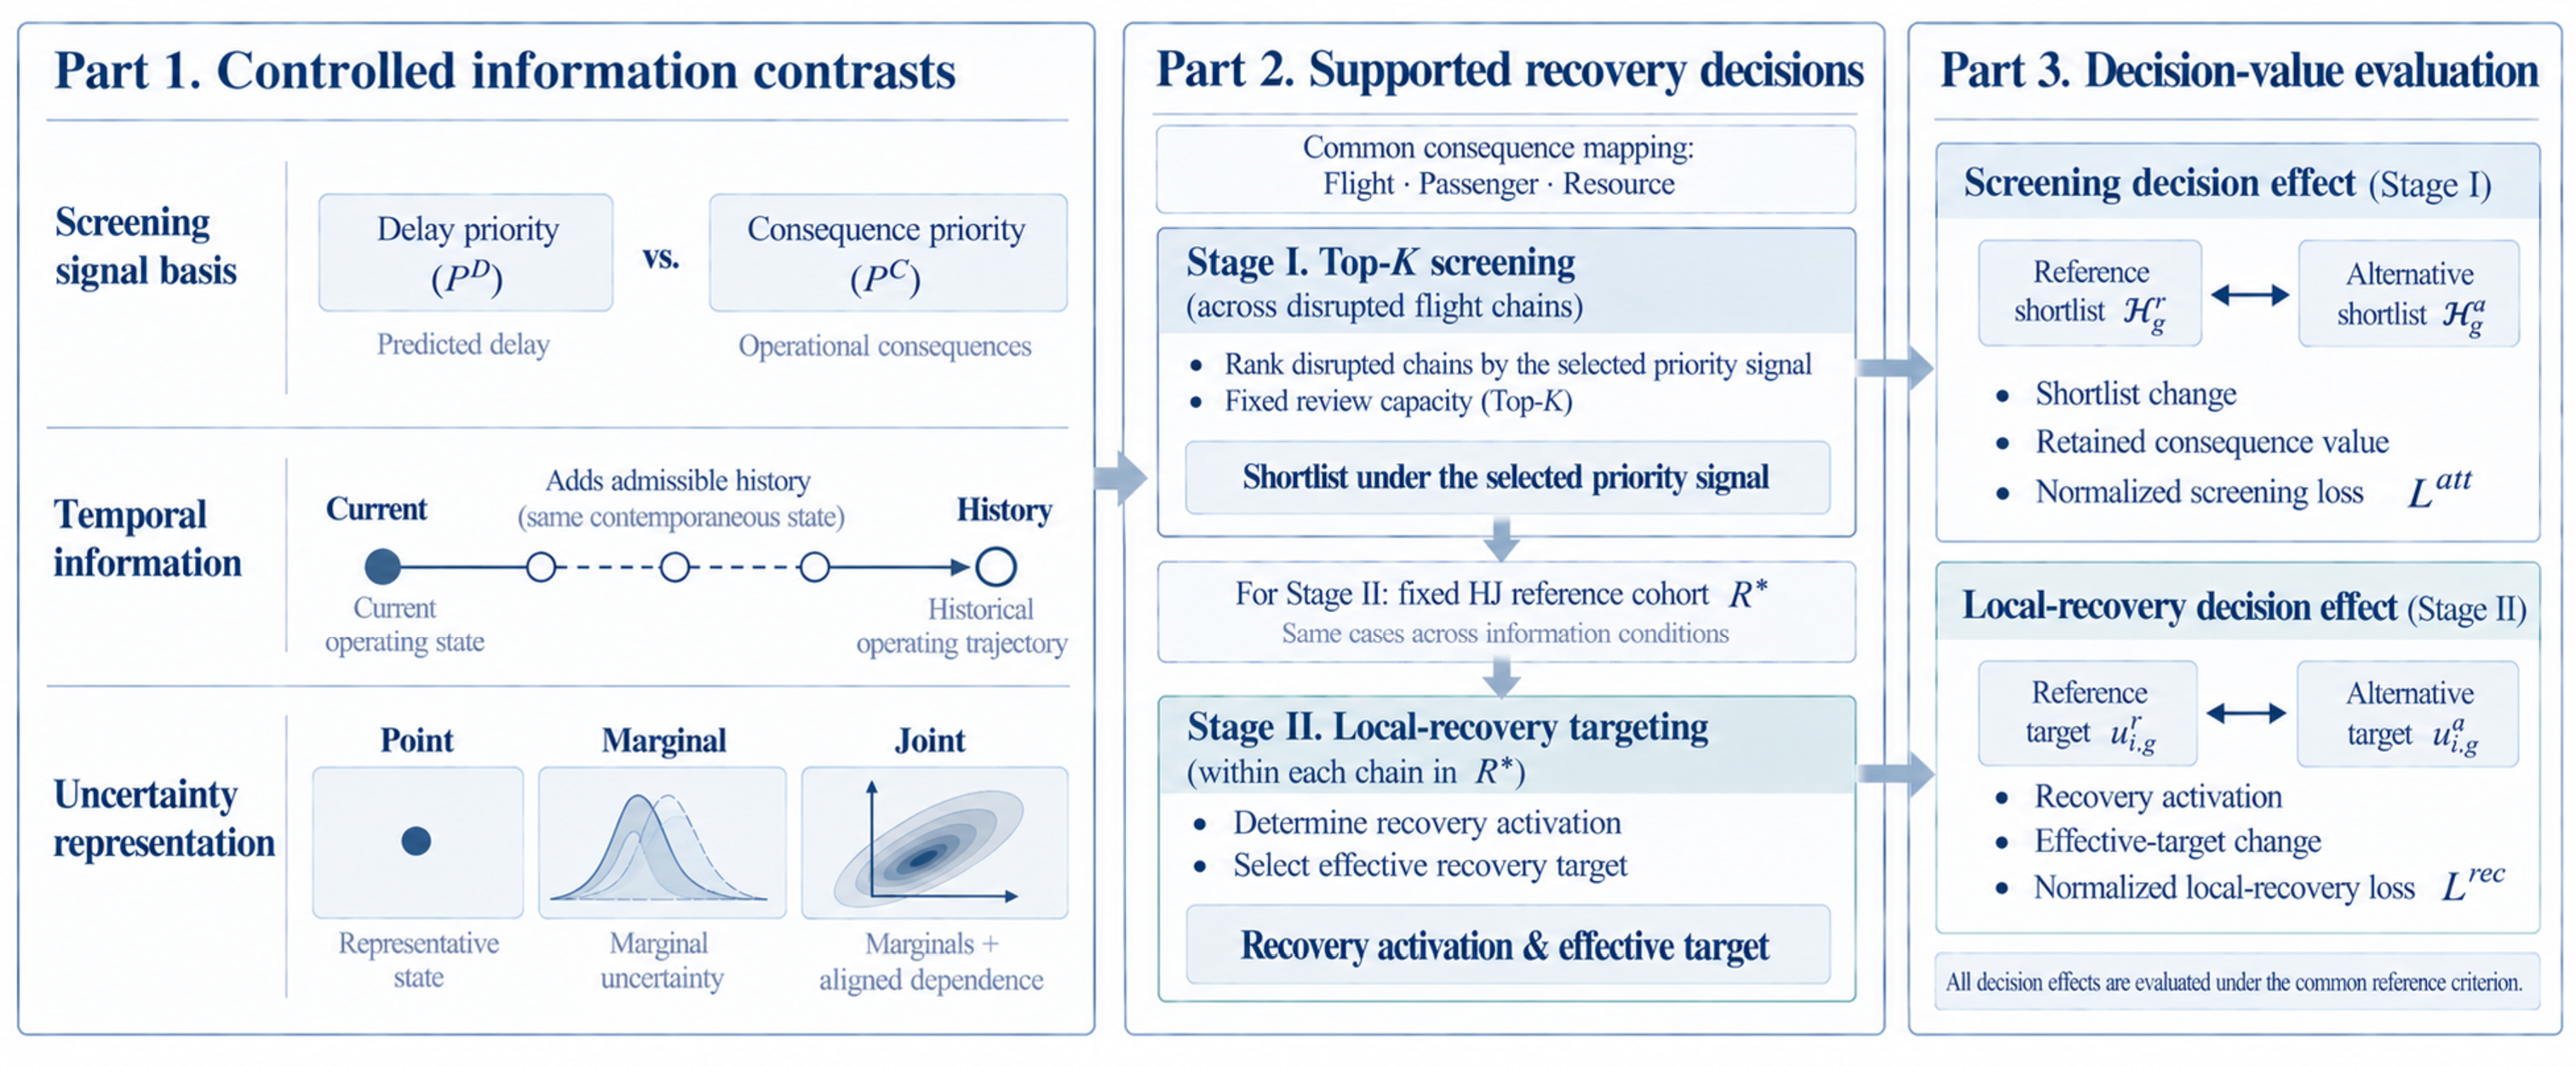
\includegraphics[width=0.98\textwidth]{figures/figure2.pdf}
    \caption{Controlled operating-information contrasts and two recovery decisions. Delay--Consequence changes the Stage-I screening signal; Current--History changes temporal representation; and Point--Marginal--Joint changes the representation of unresolved uncertainty. Stage-specific screening and within-chain recovery targeting are assessed against their respective reference decision criteria.}
    \label{fig:framework}
\end{figure}

\subsection{Aircraft-Linked Recovery Setting and Decision Contexts}
\label{subsec:decision_contexts}

We consider day-of-operation decisions in an airline operations control center (AOCC) setting. The operating unit is an aircraft-linked predecessor--successor flight chain,
\[
f_i^-\longrightarrow f_i^+.
\]
Following the predecessor's actual in-block event, the aircraft undergoes ground turnaround before operating the successor flight. A predecessor delay does not necessarily propagate to the successor by the same amount. Turnaround conditions, subsequent assignments, passenger exposure, and local operating burden all affect how delay is converted into downstream consequences. Flight chains with similar observed delays can therefore differ both in their baseline operational consequences and in their remaining recovery opportunities.

\subsubsection{Operating stages}

Four operating stages describe the progressive realization of aircraft-linked milestones. \emph{PRE} precedes the predecessor's actual in-block event, when its arrival and subsequent operating states may remain unresolved. \emph{TURN} begins after the predecessor has arrived but before the successor's actual off-block event. \emph{TAXI} follows the successor's off-block event while taxi-out and take-off remain to be completed. \emph{COMP} denotes completion of the focal operating process. As operations progress, previously uncertain milestones become factual and the unresolved state requiring prediction changes accordingly. Local off-block recovery is evaluated only at
\[
\mathcal G_A=\{\mathrm{PRE},\mathrm{TURN}\}.
\]
These operating stages govern information availability and the remaining state uncertainty. They must not be confused with Stage I and Stage II, which designate \emph{decision layers}, not operating milestones.

\subsubsection{Recovery decision contexts}

Recovery requires decisions at different managerial levels. Screening first identifies disruptions with potentially important operational consequences; detailed local assessment then considers whether an additional adjustment is worthwhile. This separation is consistent with the established distinction between disruption identification and recovery adjustment in airline recovery research \citep{peiDecisionSupportIrregular2021,zhaoTwoStageAircraftRecovery2023}. \emph{Stage I} selects chains for further diagnosis under a fixed review budget, using either delay-based or consequence-based priority. Let $z_{i,g}\in\{0,1\}$ indicate whether chain $i$ at operating stage $g$ enters the shortlist. The principal empirical comparison is a \emph{retrospective, stage-specific fixed-budget screening benchmark}: without verified concurrent candidate queues and actual AOCC review capacities, chains aggregated across different decision times are not interpreted as simultaneously competing for real review slots.

\emph{Stage II} applies to shortlisted chains with valid local-recovery support and selects an effective recovery target $u_{i,g}\in\mathcal U_{i,g}$, including zero additional recovery. This variable specifies a modeled reduction in successor operating delay rather than an executable aircraft-swap, crew-assignment, gate-allocation, or other resource-dispatch instruction. Its realized effect remains constrained by the state-dependent recovery headroom. The decision layers share an operating-state and consequence mapping but optimize different objects: Stage I compares baseline consequence exposure across chains, whereas Stage II evaluates the achievable improvement and effort associated with different targets for one chain. Accordingly, a chain with high screening priority need not have high recoverable value. Neither layer-specific optimum establishes a globally optimal, resource-coordinated airline recovery policy. The review-budget and local-target assumptions are model specifications rather than observed airline policy rules.

\subsection{Decision-Time Information and State Representations}
\label{subsec:state_representation}

Let $\mathcal E_{i,\leq t}$ denote the admissible operating evidence available for chain $i$ at or before decision epoch $t$. As milestones occur, unresolved operating events become realized facts. A separate modeling choice determines how the information that is already available is organized and represented. We therefore distinguish \emph{information availability}, \emph{temporal or distributional representation}, and the \emph{decision objective}. Altering consequence-domain preferences changes the evaluation criterion rather than the amount of operating evidence; those preferences are introduced in Section~\ref{subsec:state_consequence_decision}.

The aircraft-linked state follows the operating sequence
\[
T^{IB}_{i,t}\longrightarrow D^{OB}_{i,t}\longrightarrow D^{TX}_{i,t},
\]
where $T^{IB}$ is the predecessor in-block timing quantity, $D^{OB}$ the successor off-block delay, and $D^{TX}$ the successor's additional taxi-out delay. The arrows express operating sequence and the adopted conditional modeling order, not an identified causal effect among the variables. All three primitives may be unresolved in PRE; the predecessor in-block event is factual in TURN; and both predecessor in-block and successor off-block are factual in TAXI. Only unresolved primitives receive probabilistic predictions, while realized milestones remain fixed. The temporal origin of $T^{IB}$ and the native consequence units must be reconciled with the implementation before numerical claims are finalized.

\subsubsection{Delay baseline and operating history}

The primary scalar screening comparator is the \emph{expected successor take-off delay} conditional on decision-time evidence, rather than the successor's already realized take-off delay:
\[
P^D_{i,t}
=\mathbb E\!\left[D^{TO}_{i,t}\mid\mathcal E_{i,\leq t}\right],
\qquad
D^{TO}_{i,t}=D^{OB}_{i,t}+D^{TX}_{i,t}.
\]
Here $D^{TO}$ is the study-specific compound of off-block and additional taxi-out delays. The expected priority $P^D$ must not be confused with actual take-off delay observed only after realization. A delay signal already observed at a decision epoch, when genuinely available, is a separate empirical comparator rather than a substitute for the stated baseline.

At a common decision epoch, the \emph{Current} representation uses the contemporaneous operating-state summary and legally available frozen references. The \emph{History} representation additionally uses the admissible trajectory through the same cutoff, encoded by an operator $H_\eta$:
\[
\mathbf h_{i,t}=H_\eta\!\left(\mathcal E_{i,\leq t}\right),
\qquad
\mathcal I^H_{i,t}=\mathcal I^C_{i,t}\cup\{\mathbf h_{i,t}\}.
\]
Both representations describe the same operating process under the same information cutoff; neither may access a milestone realized after the decision. Current emphasizes the available state summary, whereas History attempts to retain aspects of delay development and state evolution not captured by that summary. The value of history is conditional: it can be redundant when the current state is sufficient for the downstream decision. Moreover, any measured difference between the implemented conditions may combine history access with changes in predictor capacity, estimation, and calibration. The comparison therefore first concerns the \emph{implemented representations}; attribution to historical evidence itself requires the matched controls described in Section~\ref{sec:implementation}.

\subsubsection{Point, Marginal, and Joint representations}

For the operating primitives unresolved at the decision epoch, \emph{Point} compresses uncertainty into one internally coherent representative state chosen by the frozen weighted-joint-medoid rule. It is not the vector of marginal means. \emph{Marginal} preserves the weighted probability distribution of each unresolved primitive while replacing the original joint coupling. \emph{Joint} preserves the original aligned, weighted scenarios and their cross-state dependence. Their conceptual sequence is
\[
\mathrm{Point}\longrightarrow\mathrm{Marginal}\longrightarrow\mathrm{Joint}.
\]
This is a sequence of retained \emph{representation features}, not successive acquisition of real observations and not an assumed ordering of decision value. Realized milestones remain identical across the representations.

To interpret a Marginal--Joint contrast specifically as the contribution of dependence, the two constructions must preserve the same \emph{weighted} one-dimensional marginal probability measures. For every unresolved primitive $S_j$ and measurable set $B$,
\begin{equation}
\Pr_{P_M}(S_j\in B)=\Pr_{P_J}(S_j\in B).
\label{eq:weighted_marginal_requirement}
\end{equation}
Preserving the coordinate values alone does not preserve their probability masses; permuting coordinate values while leaving unequal original scenario weights fixed generally violates Eq.~\eqref{eq:weighted_marginal_requirement}. The equality is a required construction-and-audit property, not a claim that the previous implementation has satisfied it. Statistical marginal preservation also does not ensure that every recombined scenario respects the temporal order and resource restrictions of airline operations. The specific coupling algorithm, weighted-mass diagnostics, and operational-support checks are therefore reported separately in the empirical implementation and supplementary documentation.

\subsection{State-Consequence-Decision Mapping}
\label{subsec:state_consequence_decision}

Each supported operating-state representation enters the same seven-component consequence mapping. The Flight domain covers aircraft continuity and turnaround pressure, successor execution delay, and downstream delay propagation. The Passenger domain covers passenger time exposure, itinerary-sensitive connection exposure, and prolonged-disruption service exposure. The Resource domain represents local operating burden through additional taxi-out delay. Write $\mathbf C_{i,g,s}(u)=(C_{i,g,s,k}(u))_{k=1}^{7}$ for the seven-dimensional consequence vector of chain $i$ at operating stage $g$, scenario $s$, and local recovery target $u$. Several components are constructed exposure proxies rather than directly observed financial losses.

Because these components have different native units, they are converted using training-period reference scales into standardized, dimensionless consequence units (CU). The criterion aggregates them first within each domain and then across domains:
\begin{equation}
\begin{aligned}
D_{i,g,s,d}(u)
&=\sum_{k\in\mathcal K_d}\alpha_{d,k}Z_{i,g,s,k}(u),\\
\Phi_{\boldsymbol\omega}\!\left(\mathbf C_{i,g,s}(u)\right)
&=\sum_{d\in\{F,P,R\}}\omega_dD_{i,g,s,d}(u).
\end{aligned}
\label{eq:consequence_criterion_sec3}
\end{equation}
Here $Z_{i,g,s,k}(u)$ denotes a standardized consequence, $\mathcal K_d$ the components assigned to domain $d$, $\alpha_{d,k}$ their fixed within-domain weights, and $\boldsymbol\omega=(\omega_F,\omega_P,\omega_R)$ the normative weights across the Flight, Passenger, and Resource domains. Under the primary \emph{Balanced} criterion, each domain receives one-third of the total weight; within Flight and Passenger, the three components receive equal within-domain shares. Thus Balanced means \emph{equal domain weights}, not equal weights for all seven components. Prespecified Flight-, Passenger-, and Resource-emphasis criteria change the managerial objective without changing the available operating evidence. Standardization addresses measurement scales, whereas weights express trade-offs among management objectives. Neither the weights nor the CU scale are inferred monetary costs or empirically elicited airline utility. Native component definitions, proxy status, and scaling rules are documented in Section~\ref{sec:implementation} and the accompanying technical material.

The same consequence mapping supports the two decision layers in different ways: Stage I compares baseline exposure across flight chains, whereas Stage II evaluates changes in the consequences of one chain after a modeled recovery adjustment and accounts for recovery effort. The two layers therefore share an evaluation framework without repeating the same optimization problem. Re-evaluating the seven components after an adjustment does not imply that every component responds to that adjustment.

\subsubsection{Fixed-budget recovery screening}

For actionable stage $g\in\mathcal G_A$, let $\mathcal N_g$ denote the candidate set under a specified screening evaluation and $K_g$ its review budget. The consequence-based priority measures the expected baseline exposure before any \emph{additional} local recovery target specified by this framework:
\[
P^C_{i,g}(\boldsymbol\omega;P_R)
=\mathbb E_{s\sim P_R}\!\left[
\Phi_{\boldsymbol\omega}\!\left(\mathbf C_{i,g,s}(0)\right)
\right].
\]
The associated screening problem is
\begin{equation}
\begin{aligned}
\max_{\{z_{i,g}\}}\quad &
\sum_{i\in\mathcal N_g}P^C_{i,g}z_{i,g}\\
\text{s.t.}\quad &
\sum_{i\in\mathcal N_g}z_{i,g}\leq K_g,\qquad
z_{i,g}\in\{0,1\}.
\end{aligned}
\label{eq:stage1_screening}
\end{equation}
With nonnegative priorities and one review slot per chain, the solution selects the $K_g$ highest-scoring candidates, using a predetermined tie-break. Replacing $P^C_{i,g}$ by $P^D_{i,g}$ changes the priority signal while retaining the same candidates, review budget, and reference consequence evaluator. The objective is to cover high-consequence disruptions for subsequent diagnosis; it does not require Stage I to have already identified the largest achievable recovery benefit for each chain. Using a fully optimized recoverable-value ranking at screening would instead assume that much of Stage-II assessment had already been undertaken. The primary quarterly evaluation remains a retrospective, stage-specific benchmark unless concurrent competition and actual capacity are independently established. PRE and TURN are not pooled into a single real-time queue. Whether a high-consequence shortlist also captures recoverable opportunities is evaluated separately.

\subsubsection{Local-recovery targeting}

For a shortlisted chain with valid local support, let $u\in\mathcal U_{i,g}$ denote a candidate effective recovery target, with $0\in\mathcal U_{i,g}$. The nominal target $u$ is distinct from the advance actually achievable in a particular state: scenario $s$ supplies nonnegative modeled recovery headroom $H_{i,g,s}$, so that
\[
r_{i,g,s}(u)=\min\{u,H_{i,g,s}\},\qquad
AOBT_{i,g,s}(u)=AOBT_{i,g,s}(0)-r_{i,g,s}(u).
\]
The first expression distinguishes the selected target from the scenario-specific realized improvement, while the second updates the successor's actual off-block time. All seven consequences are recomputed using their native response functions under the adjusted state, but some components may remain invariant. For example, if additional taxi-out delay is unchanged by the off-block adjustment, the Resource component cannot be said to improve directly. Nevertheless, changing its weight can alter the relative importance of responsive consequences and effort, thereby affecting the chosen target. For representation $R$ with conditional state distribution $P_R$, the Stage-II objective is
\begin{equation}
J_{i,g,\boldsymbol\omega}(u;P_R)
=\mathbb E_{s\sim P_R}\!\left[
\Phi_{\boldsymbol\omega}\!\left(\mathbf C_{i,g,s}(u)\right)
\right]+c_i^A(u),
\label{eq:stage2_objective_sec3}
\end{equation}
where the first term is the expected multidimensional consequence after the target is applied and $c_i^A(u)$ is a normative effort penalty for selecting that target. This term is not directly measured expenditure. The optimal target and its model-relative recoverable value are
\begin{equation}
\begin{aligned}
u^*_{i,g,\boldsymbol\omega}(P_R)
&=\argmin_{u\in\mathcal U_{i,g}}
J_{i,g,\boldsymbol\omega}(u;P_R),\\
V_{i,g,\boldsymbol\omega}(P_R)
&=J_{i,g,\boldsymbol\omega}(0;P_R)
-J_{i,g,\boldsymbol\omega}\!\left(u^*_{i,g,\boldsymbol\omega}(P_R);P_R\right).
\end{aligned}
\label{eq:stage2_opt_sec3}
\end{equation}
Ties are resolved in favor of the smaller target. As zero is always feasible, the model-optimal recoverable value is nonnegative. Yet $u^*$ is an effective local-recovery target rather than a validated resource-dispatch instruction, and $V$ is a modeled objective improvement rather than an observed economic benefit. The zero-target case excludes only \emph{additional} adjustments represented in this framework; it does not presume the absence of historical airline interventions. Likewise, the headroom restriction covers the modeled timing limits, not all crew, gate, maintenance, and airport-capacity requirements. Detailed effort parameters, physical consistency checks, and component-wise response audits are addressed in Section~\ref{sec:implementation} and the supplementary material.

\subsection{Decision Sufficiency and Incremental Decision Value}
\label{sec:incremental_decision_value}

Different information representations may change estimated operating states and expected consequences without changing the resulting recovery choice. We therefore distinguish exact decision equivalence from reference-objective loss: the former asks whether the same option is selected, while the latter assesses the consequences of any difference using a common evaluator. The loss is model-relative, not the classical ex ante value of acquiring new observations and not the causal effect of an unimplemented recovery action.

\subsubsection{Decision equivalence and reference-objective loss}

Let $R_r$ and $R_a$ be reference and alternative representations. Under the same objective weights and admissible decision sets, Stage-I outputs are the shortlists $\mathcal H_g(R)$ and Stage-II outputs are the selected targets $u^*_{i,g}(R,\boldsymbol\omega)$. Exact decision equivalence is
\begin{equation}
\begin{aligned}
R_a\sim_g^I R_r
&\iff \mathcal H_g(R_a)=\mathcal H_g(R_r),\\
R_a\sim_{i,g}^{II}R_r
&\iff u^*_{i,g}(R_a,\boldsymbol\omega)
=u^*_{i,g}(R_r,\boldsymbol\omega).
\end{aligned}
\label{eq:decision_equivalence}
\end{equation}
Decision equivalence does not require identical predicted distributions or scores. Conversely, different selections may be tied or nearly tied under the reference criterion. Selection changes and their objective consequences are therefore distinct outcomes and must be reported separately.

Let $\mathcal H_g^r$ and $\mathcal H_g^a$ be the Stage-I shortlists, with retained values
\[
A_g^r=\sum_{i\in\mathcal H_g^r}P_{i,g}^{C,r},\qquad
A_g^a=\sum_{i\in\mathcal H_g^a}P_{i,g}^{C,r}.
\]
For $A_g^r>0$, the normalized screening loss is
\[
L_g^{\mathrm{att}}=1-\frac{A_g^a}{A_g^r}.
\]
Both shortlists use the same candidate population, budget, objective weights, and reference consequence priority for evaluation. The loss is nonnegative when the reference shortlist maximizes that criterion over the common population and review capacity. Replacement counts describe how much the shortlist changes; $L_g^{\mathrm{att}}$ describes the amount of reference consequence coverage lost. Neither is a direct measure of realized airline savings.

For Stage II, let $u^r_{i,g}$ and $u^a_{i,g}$ be the two targets and evaluate both using the \emph{reference} objective $J^r_{i,g,\boldsymbol\omega}$:
\[
\Delta_{i,g,\boldsymbol\omega}^{\mathrm{rec}}
=J^r_{i,g,\boldsymbol\omega}(u^a_{i,g})
-J^r_{i,g,\boldsymbol\omega}(u^r_{i,g}).
\]
For a paired, actionable cohort $\mathcal C$, define
\begin{equation}
L^{\mathrm{rec}}(\mathcal C,\boldsymbol\omega)
=\frac{\displaystyle\sum_{(i,g)\in\mathcal C}
\Delta^{\mathrm{rec}}_{i,g,\boldsymbol\omega}}
{\displaystyle\sum_{(i,g)\in\mathcal C}
V^r_{i,g,\boldsymbol\omega}},
\label{eq:normalized_recovery_loss}
\end{equation}
only for a positive reference-value denominator and a paired cohort with common support and feasibility. The ratio is not intrinsically bounded above by one, and a zero denominator produces an undefined ratio rather than an observed zero loss. Absolute CU losses, denominator values, and supported sample sizes must accompany normalized results. Each $\boldsymbol\omega$ has its \emph{own} reference optimum and reference-value denominator; a Balanced solution cannot serve as the optimum for a different preference criterion. Zero loss under the reference representation follows by construction from its model-defined optimality and cannot establish that it is the best representation in real-world airline recovery. Stage-I and Stage-II losses also have different objects and denominators: their magnitudes should not be directly compared as if they measured a single realized benefit.

\subsubsection{Decision boundaries and representation perturbations}

The relevant comparison is across the active decision boundary. For a same-scale Stage-I comparison, write $\widetilde P_{i,g}=P_{i,g}+\delta^I_{i,g}$. Define the reference cutoff margin and the maximum relative perturbation across selected and unselected cases by
\[
\begin{aligned}
m_g&=\min_{i\in\mathcal H_g^r,\,j\notin\mathcal H_g^r}
(P_{i,g}-P_{j,g}),\\
\Delta_g^I&=\max_{i\in\mathcal H_g^r,\,j\notin\mathcal H_g^r}
\left|\delta^I_{i,g}-\delta^I_{j,g}\right|.
\end{aligned}
\]
A sufficient condition for an unchanged shortlist is
\begin{equation}
\Delta_g^I<m_g\quad\Longrightarrow\quad\mathcal H_g^a=\mathcal H_g^r.
\label{eq:stage1_stability}
\end{equation}
For Stage II, let $u^r_{i,g}$ be the reference optimum, $\gamma_{i,g}$ the smallest reference-objective gap to another feasible target, and $\delta^{II}_{i,g}(u)$ the alternative-minus-reference objective perturbation. Define
\[
\begin{aligned}
\gamma_{i,g}&=\min_{u\in\mathcal U_{i,g},\,u\ne u^r_{i,g}}
\bigl[J^r_{i,g}(u)-J^r_{i,g}(u^r_{i,g})\bigr],\\
\Delta_{i,g}^{II}&=\max_{u\in\mathcal U_{i,g},\,u\ne u^r_{i,g}}
\left|\delta^{II}_{i,g}(u)-\delta^{II}_{i,g}(u^r_{i,g})\right|.
\end{aligned}
\]
Then
\begin{equation}
\Delta_{i,g}^{II}<\gamma_{i,g}
\quad\Longrightarrow\quad u^a_{i,g}=u^r_{i,g}.
\label{eq:stage2_stability}
\end{equation}
These are standard \emph{sufficient}, not necessary, stability conditions; failure of a certificate does not imply that a choice changes. Tie cases and singleton feasible sets follow the common decision rules and are documented with the derivations in the Supplementary Material. Both conditions concern comparable, same-scale objective perturbations. Raw delay minutes and normalized consequence scores are not on a common scale, so the Delay--Consequence comparison must be evaluated through selected shortlists and retained reference value rather than direct score subtraction.

\subsubsection{Decision objectives and distributional dependence}

Let $P_J$ and $P_M$ be Joint and valid Marginal couplings with identical weighted primitive marginals, the same target set, and the same effort specification. Define the objective difference for a fixed target $u$:
\begin{equation}
\begin{aligned}
e_{\boldsymbol\omega}(u)
&=J_{\boldsymbol\omega}(u;P_J)
-J_{\boldsymbol\omega}(u;P_M)\\
&=\sum_{d\in\{F,P,R\}}\omega_d
\left[\mathbb E_{P_J}D_d(u,S)
-\mathbb E_{P_M}D_d(u,S)\right].
\end{aligned}
\label{eq:dependence_objective_difference}
\end{equation}
An individual objective-level difference need not alter the preferred target. Let $u_J^*$ minimize $J_{\boldsymbol\omega}(\cdot;P_J)$ and, for another candidate $v$, define $g_{J,\boldsymbol\omega}(v)=J_{\boldsymbol\omega}(v;P_J)-J_{\boldsymbol\omega}(u_J^*;P_J)$. Algebraically,
\begin{equation}
\begin{aligned}
&J_{\boldsymbol\omega}(v;P_M)
-J_{\boldsymbol\omega}(u_J^*;P_M)\\
&\quad=g_{J,\boldsymbol\omega}(v)
-\bigl[e_{\boldsymbol\omega}(v)-e_{\boldsymbol\omega}(u_J^*)\bigr].
\end{aligned}
\label{eq:relative_dependence_perturbation}
\end{equation}
Thus, if
\[
e_{\boldsymbol\omega}(v)-e_{\boldsymbol\omega}(u_J^*)
>g_{J,\boldsymbol\omega}(v),
\]
Marginal strictly prefers $v$ to the original Joint-optimal target $u_J^*$; equality is governed by the fixed tie-break. The condition does not assert that $v$ must be Marginal's global optimum. Dependence can alter the absolute evaluation of every candidate yet leave the preferred target unchanged if those evaluations shift by the same constant. What matters for selection is the \emph{difference in dependence perturbations across feasible targets}, compared with the original objective gap. Domain weights determine the relative importance of consequences, while cross-state interactions determine which dependence patterns affect those consequences. Changing weights alone does not guarantee any new dependence sensitivity: a domain invariant to $u$ may affect the balance between responsive domains and effort without providing a direct improvement in that domain. These relationships provide conditional mechanisms for objective-by-distribution comparisons rather than novel general optimization theorems or predetermined empirical findings.

\subsubsection{Conditions for marginal sufficiency}

A limiting benchmark establishes one condition under which marginal information is sufficient. Suppose that, for each fixed feasible target $u$, the complete consequence criterion is additive across unresolved primitive states; the Marginal and Joint representations have identical weighted one-dimensional marginals; and both use the same distribution-independent feasible set and recovery-effort term. Then
\begin{equation}
J_{\boldsymbol\omega}(u;P_J)
=J_{\boldsymbol\omega}(u;P_M),\qquad
\forall u\in\mathcal U.
\label{eq:separable_marginal_sufficiency}
\end{equation}
The expected evaluation of each fixed feasible target is therefore identical, and the selected optimum also coincides under a common tie-break. This is a sufficient condition for marginal sufficiency, not a necessary condition: even a nonadditive consequence may yield identical decisions when its relative perturbation cancels across candidates. Airline recovery may depart from separability because off-block and taxi-out delays jointly enter threshold-based passenger or service exposures, while scenario-dependent headroom couples predecessor in-block timing with successor off-block timing. These mechanisms make additional dependence value \emph{possible}, but they do not guarantee a different optimum. Their effects must be established through valid empirical comparisons rather than asserted from the existence of coupling alone.

As operations roll forward, both the evidence available to the decision maker and the remaining headroom or feasible recovery set may change. Decisions at different epochs therefore do not necessarily concern the same optimization problem. Their differences should be analyzed separately from fixed-epoch representation contrasts and must not, by themselves, be interpreted as causal gains from information revelation.
